\chapter{摩尔与摩尔质量}\label{ch:g10:the-mole}

归根结底，银行数硬币并不是一枚一枚地数，
而是称其质量。若一枚硬币的质量为 \qty{7.5}{g}，
一袋质量为 \qty{7.5}{kg} 的硬币恰好是一千枚，
秤已替我们完成了计数。化学家面对的是同样的问题，
只是原子的数目要多得多：一小勺水所含的分子数，
超过海岸上所有沙滩的沙粒数。他们的办法同样是称重，
而他们所用的“袋子”能装下
\num{602214076000000000000000} 个微粒。本章定义这个“袋子”，
即摩尔，并说明如何由天平上的质量求出
原子或分子的个数。

\begin{recall}
原子的质量集中在其原子核上；质子与中子各自的质量约为
\qty{1.67e-27}{kg}，因此质量数为 $A$ 的原子的质量约为
$A \times \qty{1.67e-27}{kg}$。大数与小数
用科学记数法表示
（见\cref{ch:g9:inside-the-atom}）。化学式给出分子中
每种元素的原子个数（见\cref{ch:g7:atoms-and-molecules}）。
\end{recall}

\begin{omfigure}
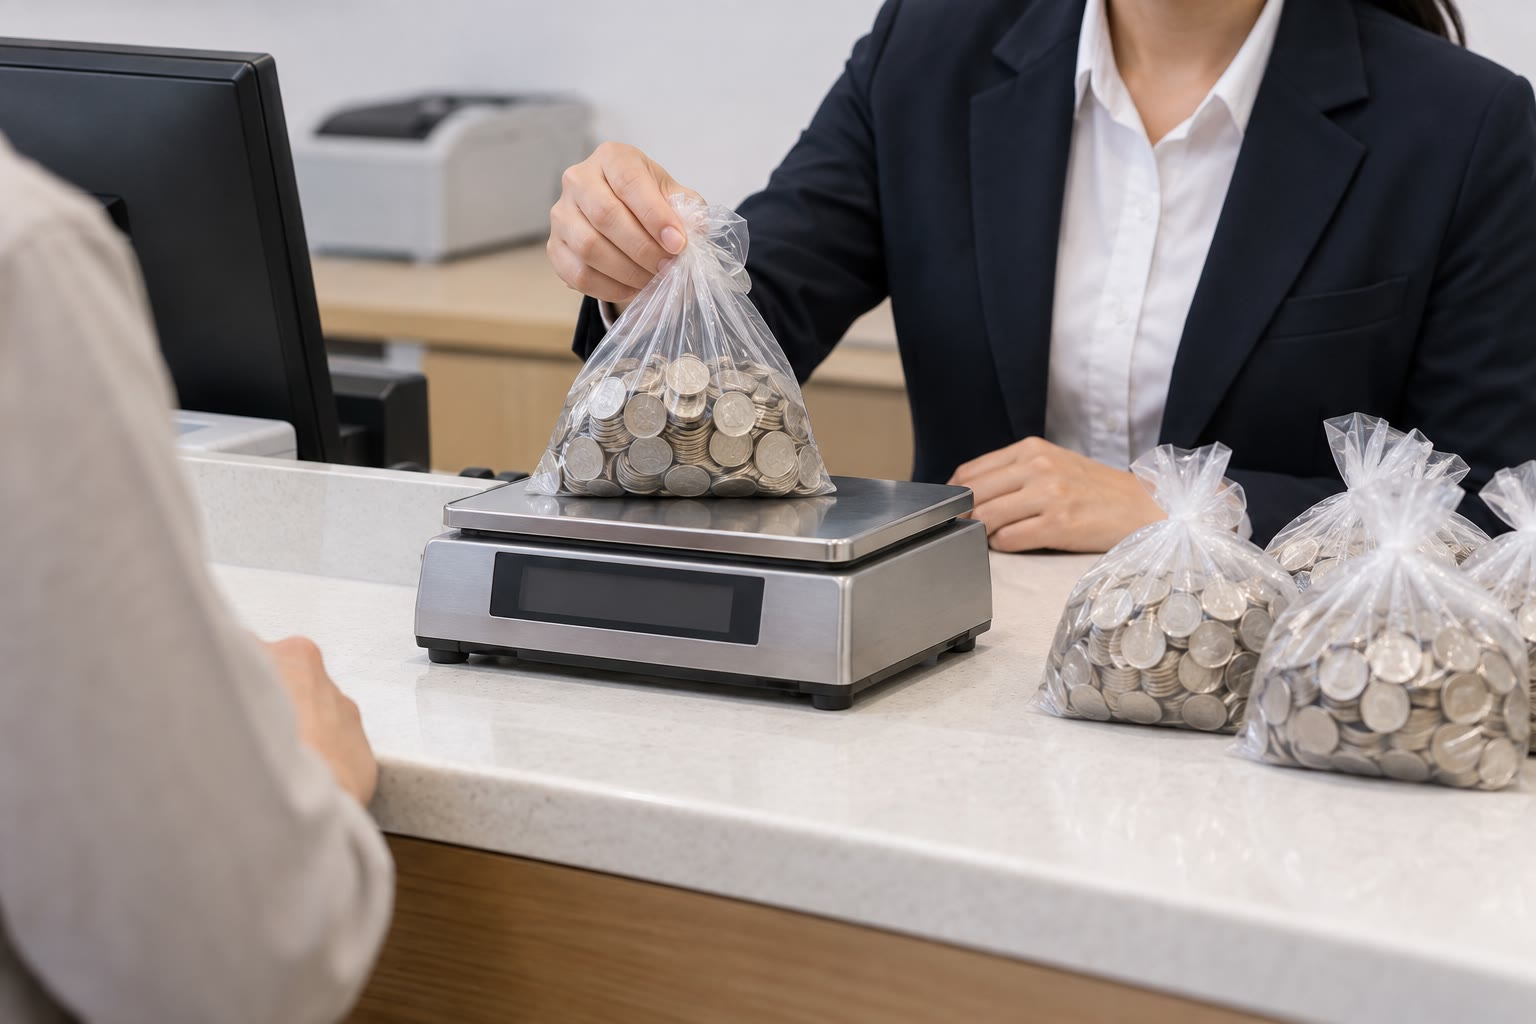
\includegraphics[width=0.55\linewidth]{images/book1/ai/g10-bank-coins.jpg}

{\small 银行通过称重来数硬币，化学家数原子的方法
与此相同。}
\end{omfigure}

\section{通过称重计数}

\begin{example}[一袋硬币]\label{ex:g10:the-mole:coins}
一枚硬币的质量为 \qty{7.5}{g}。一袋这样的硬币的质量为
\qty{1.80}{kg}，即 \qty{1800}{g}（不计袋子本身的质量）。
它所含硬币的枚数为
\[
  \frac{\qty{1800}{g}}{\qty{7.5}{g}} = 240 \text{ 枚硬币。}
\]
计数时，银行用总质量除以一枚硬币的质量。
\end{example}

\begin{example}[一小勺水]\label{ex:g10:the-mole:spoon}
水分子 \ce{H2O} 含有 $2 + 16 = 18$ 个核子（氧-16
和氢-1 原子几乎构成了天然水的全部），因此其质量约为
$18 \times \qty{1.67e-27}{kg} = \qty{3.0e-26}{kg}$，即
\qty{3.0e-23}{g}。一小勺 \qty{5.0}{g} 的水因此含有
\[
  \frac{\qty{5.0}{g}}{\qty{3.0e-23}{g}} \approx \num{1.7e23}
  \text{ 个分子。}
\]
这种除法与硬币的情形相同，但结果是
一个无人能够想象的数字。化学家需要
与实验室样品大小相适应的一种微粒“包装”。
\end{example}

\begin{definition}[物质的量与摩尔]\label{def:g10:the-mole:amount}
% ledger: const:NA
样品的\emph{物质的量}\index{物质的量} $n$ 表示其
所含微粒（原子、分子或离子，每次需注明）的数目。
其单位为\emph{摩尔}\index{摩尔}，符号为 \si{mol}：一摩尔
恰好含有 \num{6.02214076e23} 个微粒。
\end{definition}

\begin{remark}[一打、一令与一摩尔]\label{rem:g10:the-mole:dozen}
摩尔是一个计数单位，与一打鸡蛋（12 个）或
一令纸（500 张）类似，只是大得多。“两摩尔水分子”
表示 $2 \times \num{6.02214076e23} = \num{1.20e24}$ 个分子，正如
“两打鸡蛋”表示 24 个鸡蛋。务必说明所计数的是哪种微粒：
一摩尔氧\emph{分子} \ce{O2} 含有两摩尔氧
\emph{原子}。
\end{remark}

\begin{history}[阿伏伽德罗假说，1811 年]
1811 年，物理学家阿伏伽德罗提出：
在相同的温度和压强下，相同体积的不同气体
含有相同数目的粒子。他还认识到，氧气等气体
是由两个原子构成的分子。他的思想被忽视了
近五十年，直到 1860 年斯坦尼斯劳·坎尼扎罗用它得到了
一套相互协调的原子量。表示一摩尔所含微粒数的常数
后来以阿伏伽德罗命名，而他从未知道其数值。
\end{history}

\begin{omfigure}
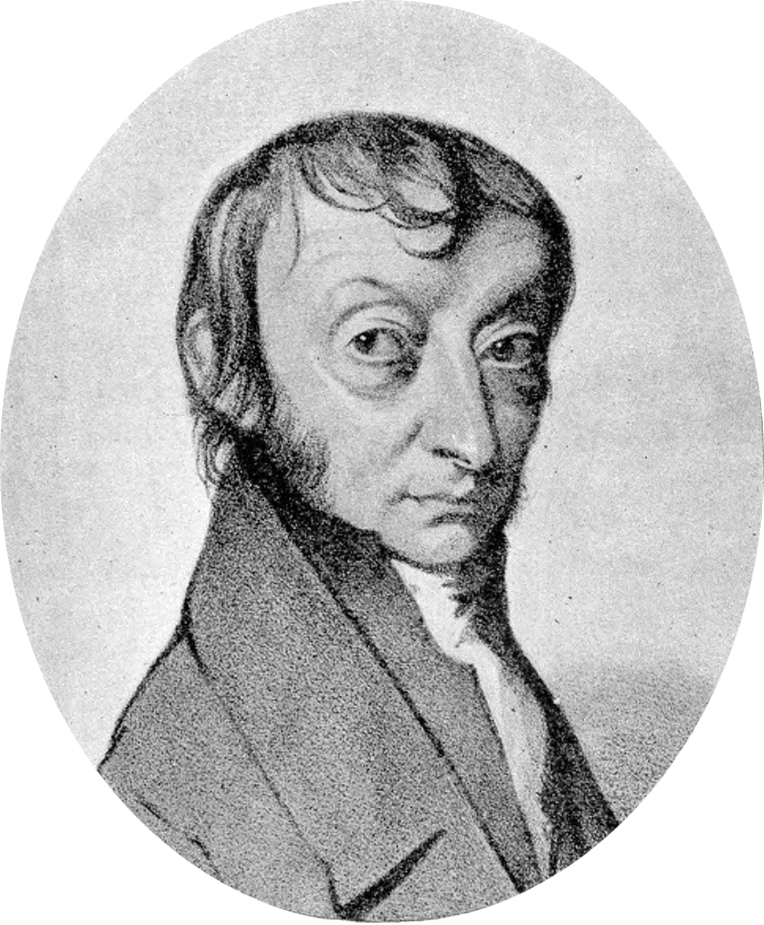
\includegraphics[width=0.26\linewidth]{images/book1/avogadro.jpg}

{\small 阿伏伽德罗（1776--1856）。}
\end{omfigure}

\section{阿伏伽德罗常数}

\begin{definition}[阿伏伽德罗常数]\label{def:g10:the-mole:avogadro}
% ledger: const:NA
\emph{阿伏伽德罗常数}\index{阿伏伽德罗常数} $N_A$ 是
每摩尔所含的微粒数：
\[
  N_A = \qty{6.02214076e23}{mol^{-1}} .
\]
其数值是精确的，由定义确定。计算时
取近似值 \qty{6.02e23}{mol^{-1}}。
\end{definition}

\begin{proposition}[微粒数与物质的量]\label{prop:g10:the-mole:number}
含有 $N$ 个微粒的样品，其物质的量为
\[
  n = \frac{N}{N_A}, \qquad\text{即}\qquad N = n \times N_A .
\]
\end{proposition}

\begin{proof}
每摩尔含有 $N_A$ 个微粒，因此 $n$ 摩尔含有 $n \times N_A$
个微粒；两边除以 $N_A$ 即得 $n$。
\end{proof}

\begin{example}[分子与摩尔]\label{ex:g10:the-mole:convert}
一份样品含有 \num{1.5e24} 个二氧化碳分子，其
物质的量为
$n = \num{1.5e24} / \qty{6.02e23}{mol^{-1}} = \qty{2.5}{mol}$.
反之，\qty{0.20}{mol} 铁含有
$N = \qty{0.20}{mol} \times \qty{6.02e23}{mol^{-1}} = \num{1.2e23}$
个铁原子。
\end{example}

\begin{remark}[数值的来源]\label{rem:g10:the-mole:origin}
五十多年间，摩尔曾被定义为
恰好 \qty{12}{g} 碳-12 中的原子数，而 $N_A$ 须经测量确定。
自 2019 年起，该数值本身已被固定，使摩尔成为纯粹的计数单位。
新旧两种定义的一致程度优于
亿分之一，因此十二克碳-12 仍含有一摩尔
原子，如下一节所验证。
\end{remark}

\section{摩尔质量}

\begin{definition}[摩尔质量]\label{def:g10:the-mole:molar-mass}
化学物种的\emph{摩尔质量}\index{摩尔质量} $M$ 是
一摩尔该物种所含微粒的质量，单位为克每摩尔（\si{g/mol}）。
元素按其天然同位素混合物取平均所得的摩尔质量，
即其\emph{原子的摩尔质量}\index{原子的摩尔质量}；
它印在元素周期表中。
\end{definition}

\begin{example}[一摩尔碳原子]\label{ex:g10:the-mole:carbon}
% ledger: const:NA, const:u
一个碳-12 原子的质量约为
$12 \times \qty{1.67e-27}{kg} = \qty{2.00e-26}{kg}$。一摩尔这样的原子
的质量为
\[
  \qty{2.00e-26}{kg} \times \num{6.02e23} = \qty{1.20e-2}{kg}
  = \qty{12.0}{g}.
\]
摩尔的取值使得原子的摩尔质量（以克每
摩尔计）的数值接近其质量数：氢约为 \qty{1}{g/mol}，
碳为 \qty{12}{g/mol}，氧为 \qty{16}{g/mol}。
\end{example}

\begin{omfigure}
% ledger: aw:H, aw:C, aw:N, aw:O, aw:Na, aw:Mg, aw:Al, aw:Si, aw:S, aw:Cl, aw:K, aw:Ca, aw:Fe, aw:Cu, aw:Zn, aw:Au (rounded to 0.1)
\begin{tabular}{lcr@{\qquad}lcr}
\hline
元素 & 符号 & $M$（\si{g/mol}） & 元素 & 符号 & $M$（\si{g/mol}） \\
\hline
氢  & \ce{H}  & 1.0  & 硅   & \ce{Si} & 28.1 \\
碳    & \ce{C}  & 12.0 & 硫    & \ce{S}  & 32.1 \\
氮  & \ce{N}  & 14.0 & 氯  & \ce{Cl} & 35.5 \\
氧    & \ce{O}  & 16.0 & 钾    & \ce{K}  & 39.1 \\
钠    & \ce{Na} & 23.0 & 钙    & \ce{Ca} & 40.1 \\
镁 & \ce{Mg} & 24.3 & 铁 & \ce{Fe} & 55.8 \\
铝 & \ce{Al} & 27.0 & 铜 & \ce{Cu} & 63.5 \\
          &   &   & 金 & \ce{Au} & 197.0 \\
\hline
\end{tabular}\par\medskip

{\small 常见元素的原子摩尔质量，精确到
\qty{0.1}{g/mol}。本书采用这些数值。}
\end{omfigure}

\begin{remark}[氯为何是 35.5]\label{rem:g10:the-mole:chlorine}
% ledger: iso:Cl35, iso:Cl37
天然氯是两种同位素的混合物：约四分之三的
原子为氯-35，四分之一为氯-37
（见\cref{ch:g9:inside-the-atom}）。其原子的摩尔质量是
按这些比例加权平均所得的值，介于 35 与 37 之间：\qty{35.5}{g/mol}。
这也是部分原子摩尔质量远非整数的原因。
\end{remark}

\begin{proposition}[分子的摩尔质量]\label{prop:g10:the-mole:sum}
分子的摩尔质量，等于化学式中各原子的
原子摩尔质量之和，每个原子按其在化学式中出现的次数计入。
同样的规则可由离子型固体的化学式单位求出其摩尔质量。
\end{proposition}

\begin{proof}
一摩尔 \ce{A_xB_y} 分子含有 $x$ 摩尔 \ce{A} 原子和
$y$ 摩尔 \ce{B} 原子，且不含其他成分；其质量为二者
质量之和，即 $x\,M(\ce{A}) + y\,M(\ce{B})$。
\end{proof}

\begin{example}[三种物质的摩尔质量]\label{ex:g10:the-mole:three}
% ledger: aw:H, aw:C, aw:O, aw:Na, aw:Cl
\begin{align*}
  M(\ce{H2O}) &= 2 \times 1.0 + 16.0 = \qty{18.0}{g/mol},\\
  M(\ce{NaCl}) &= 23.0 + 35.5 = \qty{58.5}{g/mol},\\
  M(\ce{C12H22O11}) &= 12 \times 12.0 + 22 \times 1.0 + 11 \times 16.0
     = \qty{342.0}{g/mol}.
\end{align*}
最后一个是蔗糖，即食用糖。
\end{example}

\section{由质量到物质的量及其逆运算}

\begin{proposition}[质量与物质的量]\label{prop:g10:the-mole:mass}
质量为 $m$、摩尔质量为 $M$ 的某种物质的样品，所含物质的量为
\[
  n = \frac{m}{M}, \qquad\text{即}\qquad m = n \times M .
\]
若 $m$ 以克计，$M$ 以克每摩尔计，则 $n$ 的单位为摩尔。
\end{proposition}

\begin{proof}
每摩尔的质量为 $M$，故 $n$ 摩尔的质量为 $n \times M$；
这相当于银行清点硬币，只不过以摩尔作一枚硬币。
\end{proof}

\begin{method}[由质量求粒子数]\label{met:g10:the-mole:mass-to-number}
\begin{enumerate}
  \item 写出该物质的化学式，
        并由表中查得其摩尔质量 $M$。
  \item 必要时将质量换算为克，然后计算 $n = m / M$。
  \item 若需求粒子数，则 $N = n \times N_A$。
  \item 检查数量级：几克小分子约为
        十分之一摩尔的量级，即约 $10^{22}$ 至 $10^{23}$
        个粒子。
\end{enumerate}
\end{method}

\begin{omfigure}
\begin{tikzpicture}[font=\small, box/.style={draw=omDef, very thick,
    fill=omDef!8, rounded corners=3pt, minimum width=2.9cm,
    minimum height=1.1cm, align=center}]
  \node[box] (m) at (0,0) {质量 $m$\\[1pt] (\si{g})};
  \node[box] (n) at (5,0) {物质的量 $n$\\[1pt] (\si{mol})};
  \node[box] (N) at (10,0) {粒子数 $N$\\[1pt] （个）};
  \draw[-{Stealth[length=7pt]}, thick, omProp] ([yshift=4pt]m.east)
    -- node[above] {$\div M$} ([yshift=4pt]n.west);
  \draw[-{Stealth[length=7pt]}, thick, omProp] ([yshift=-4pt]n.west)
    -- node[below] {$\times M$} ([yshift=-4pt]m.east);
  \draw[-{Stealth[length=7pt]}, thick, omProp] ([yshift=4pt]n.east)
    -- node[above] {$\times N_A$} ([yshift=4pt]N.west);
  \draw[-{Stealth[length=7pt]}, thick, omProp] ([yshift=-4pt]N.west)
    -- node[below] {$\div N_A$} ([yshift=-4pt]n.east);
\end{tikzpicture}

{\small 物质的量 $n$ 居中：天平给出 $m$，
由摩尔质量得到 $n$，再由阿伏伽德罗常数
得到粒子数。}
\end{omfigure}


\begin{example}[9 克水]\label{ex:g10:the-mole:nine}
% ledger: aw:H, aw:O, const:NA
\qty{9.0}{g} 水中有多少个分子？$M(\ce{H2O}) =
\qty{18.0}{g/mol}$，故
\[
  n = \frac{\qty{9.0}{g}}{\qty{18.0}{g/mol}} = \qty{0.50}{mol},
  \qquad
  N = \qty{0.50}{mol} \times \qty{6.02e23}{mol^{-1}}
    = \num{3.0e23} \text{ 个分子。}
\]
\end{example}

\begin{example}[桌上的一摩尔]\label{ex:g10:the-mole:bench}
% ledger: rho:water, rho:NaCl, rho:sucrose, rho:Fe, aw:H, aw:O, aw:Na, aw:Cl, aw:C, aw:Fe
一摩尔水重 \qty{18.0}{g}，约一汤匙。一摩尔食盐，
\qty{58.5}{g}，是一小堆；一摩尔蔗糖重 \qty{342.0}{g}，可
装满一个马克杯；一摩尔铁重 \qty{55.8}{g}，是一个边长略小于
\qty{2}{cm} 的立方体。四者所含粒子数相同：
蔗糖分子只是比水分子重得多，而铁原子
排列得紧密得多。
\end{example}

\begin{omfigure}
\begin{tikzpicture}[font=\small, x=0.62cm, y=0.62cm]
  % cubes of true volume, drawn to one common scale: side = cube root of V
  % water 18.09 cm3 -> 2.625 cm; NaCl 26.96 cm3 -> 2.999 cm;
  % sucrose 216.4 cm3 -> 6.004 cm; Fe 7.09 cm3 -> 1.921 cm
  \newcommand{\cube}[4]{% x, side, fill, label
    \pgfmathsetmacro\d{0.35*#2}
    \fill[#3!35, draw=#3!80!black] (#1,0) rectangle ++(#2,#2);
    \fill[#3!20, draw=#3!80!black] (#1,#2) -- ++(\d,\d) -- ++(#2,0)
      -- ++(-\d,-\d) -- cycle;
    \fill[#3!50, draw=#3!80!black] (#1+#2,0) -- ++(\d,\d) -- ++(0,#2)
      -- ++(-\d,-\d) -- cycle;
    \node[below, align=center] at (#1+#2/2,-0.1) {#4};}
  \cube{0}{2.625}{cyan}{water\\ \qty{18.0}{g}\\ \qty{18}{cm^3}}
  \cube{4.3}{2.999}{gray}{salt\\ \qty{58.5}{g}\\ \qty{27}{cm^3}}
  \cube{9}{6.004}{orange}{sugar\\ \qty{342.0}{g}\\ \qty{216}{cm^3}}
  \cube{18}{1.921}{brown}{iron\\ \qty{55.8}{g}\\ \qty{7}{cm^3}}
\end{tikzpicture}

{\small 水、食盐（氯化钠）、蔗糖和铁各一摩尔，
按其真实体积画成立方体，所有图形比例相同。
每份均含 \num{6.02e23} 个粒子。}
\end{omfigure}

\section{气体：摩尔体积}

\begin{definition}[摩尔体积]\label{def:g10:the-mole:molar-volume}
气体的\emph{摩尔体积}\index{摩尔体积} $V_m$ 是指
在给定温度和压强下，一摩尔该气体所占的体积。
其单位为升每摩尔（\si{L/mol}）。
\end{definition}

\begin{proposition}[所有气体的摩尔体积相同]\label{prop:g10:the-mole:avogadro-law}
% ledger: const:R, const:atm, const:Vm1 (24.1 = R x 293.15 K / 101325 Pa, computed)
在给定温度和压强下，任何气体一摩尔所占的体积
几乎相同，与气体种类无关。在 \qty{20}{\celsius} 和
标准大气压强下，
\[
  V_m = \qty{24.1}{L/mol};
\]
在 \qty{0}{\celsius}、同一压强下，$V_m = \qty{22.4}{L/mol}$。
体积为 $V$ 的气体，其物质的量为 $n = V / V_m$。
\end{proposition}

\begin{proof}
此处不加证明地承认：这是阿伏伽德罗于 1811 年提出的假设，
现已成为物理定律，而 $V_m$ 的数值由
物理教材中所学的气体定律推出。
\end{proof}

\begin{omfigure}
\begin{tikzpicture}[font=\small]
  \foreach \x/\g/\m/\c in {0/{\ce{H2}}/2.0/cyan, 4/{\ce{O2}}/32.0/red,
                           8/{\ce{CO2}}/44.0/gray} {
    \draw[thick, black!60] (\x,-0.25) -- (\x,-1.1);
    \shade[ball color=\c!45, draw=\c!70!black] (\x,0.55) ellipse (1.05 and 1.2);
    \fill[\c!70!black] (\x-0.12,-0.68) -- (\x+0.12,-0.68) -- (\x,-0.55) -- cycle;
    \node[align=center] at (\x,-1.65) {1 摩尔 \g\\ \qty{\m}{g},
      \qty{24.1}{L}};
  }
\end{tikzpicture}

{\small 三个气球处于 \qty{20}{\celsius}，每个都装有一摩尔
不同的气体。它们的体积相同，质量却不同。}
\end{omfigure}


\begin{example}[一个装有二氧化碳的气球]\label{ex:g10:the-mole:balloon}
% ledger: aw:C, aw:O
一个气球在 \qty{20}{\celsius} 下装有 \qty{2.4}{L} 二氧化碳。
其物质的量为 $n = \qty{2.4}{L} / \qty{24.1}{L/mol} = \qty{0.10}{mol}$，
其质量 $m = \qty{0.10}{mol} \times \qty{44.0}{g/mol} =
\qty{4.4}{g}$。同一气球若充满氢气，则所含
物质的量同为 \qty{0.10}{mol}，但气体质量仅 \qty{0.20}{g}。
\end{example}

\begin{remark}[重气体与轻气体]\label{rem:g10:the-mole:heavy}
由于任何气体一升所含的物质的量相同，一升气体的质量
与其摩尔质量成正比。空气是约五分之四的氮气
（\qty{28.0}{g/mol}）与五分之一的氧气
（\qty{32.0}{g/mol}）组成的混合物，其行为相当于摩尔质量约为
\qty{29}{g/mol}的气体。摩尔质量较大的气体，如二氧化碳
（\qty{44.0}{g/mol}），密度大于空气，会聚集在密闭地窖的底部；
摩尔质量较小的气体，如氦气
（\qty{4.0}{g/mol}），则会上升。
\end{remark}

\section{练习}

\begin{exercise}[$\star$]\label{exo:g10:the-mole:1}
求下列物质的摩尔质量：氧气 \ce{O2}、氮气 \ce{N2}、
甲烷 \ce{CH4}、氨 \ce{NH3} 和二氧化碳 \ce{CO2}。
\end{exercise}

\begin{exercise}[$\star$]\label{exo:g10:the-mole:2}
\qty{36.0}{g} 水中含有多少物质的量？
\qty{4.0}{g} 甲烷中含有多少？
\end{exercise}

\begin{exercise}[$\star$]\label{exo:g10:the-mole:3}
\qty{0.25}{mol} 氯化钠 \ce{NaCl} 的质量是多少？
\qty{2.0}{mol} 二氧化碳的质量呢？
\end{exercise}

\begin{exercise}[$\star$]\label{exo:g10:the-mole:4}
\qty{0.50}{mol} 氧气中有多少个分子？
含 \num{3.0e24} 个铁原子的铁，其物质的量是多少？
\end{exercise}

\begin{exercise}[$\star$]\label{exo:g10:the-mole:5}
在 \qty{20}{\celsius} 和标准大气压下，
\qty{0.50}{mol} 氮气占据多大体积？在该气体
\qty{12}{L} 中含有多少物质的量的氧气？
\end{exercise}

\begin{exercise}[$\star\star$]\label{exo:g10:the-mole:6}
一滴水的体积为 \qty{0.050}{mL}，而 \qty{1}{mL} 水
的质量为 \qty{1.0}{g}。这一滴水中
含有多少个水分子？
\end{exercise}

\begin{exercise}[$\star\star$]\label{exo:g10:the-mole:7}
哪种物质所含原子更多：\qty{10}{g} 铝还是 \qty{10}{g}
铁？先不经计算说明理由，再通过计算加以检验。
\end{exercise}

\begin{exercise}[$\star\star$]\label{exo:g10:the-mole:8}
在 \qty{20}{\celsius} 下，求一升二氧化碳
和一升氮气的质量。为什么二氧化碳会聚集在
正在发酵葡萄汁的密闭地窖底部？
\end{exercise}

\begin{exercise}[$\star\star$]\label{exo:g10:the-mole:9}
利用三个方框 $m$、$n$、$N$ 的图示，求
\num{1.0e22} 个葡萄糖 \ce{C6H12O6} 分子的质量。
请写出所依循的两个箭头。
\end{exercise}

\begin{exercise}[$\star\star$]\label{exo:g10:the-mole:10}
一块糖（蔗糖，\ce{C12H22O11}）的质量为 \qty{5.0}{g}。
求其中所含蔗糖的物质的量，再求蔗糖
分子数，然后求碳原子数。
\end{exercise}

\begin{exercise}[$\star\star$]\label{exo:g10:the-mole:11}
哪一种所含分子的物质的量更多：\qty{1.0}{kg} 水
\ce{H2O}，还是 \qty{1.0}{kg} 乙醇 \ce{C2H6O}？相差多少倍？
\end{exercise}

\begin{exercise}[$\star\star\star$]\label{exo:g10:the-mole:12}
一枚金戒指的质量为 \qty{5.0}{g}，其中四分之三为
金，其余为铜。它含有多少个金原子？多少个
铜原子？戒指中哪种金属的原子更多？
\end{exercise}

\begin{exercise}[$\star\star\star$]\label{exo:g10:the-mole:13}
一间教室长 \qty{8.0}{m}、宽 \qty{6.0}{m}、高 \qty{3.0}{m}，
室内空气温度为 \qty{20}{\celsius}。
\begin{enumerate}
  \item 求其中所含气体的物质的量（$\qty{1}{m^3} =
        \qty{1000}{L}$）？分子数是多少？
  \item 设空气中每一百个分子中有 78 个氮气分子、21 个氧气分子、1 个
        氩（\qty{40.0}{g/mol}），求空气的平均
        摩尔质量。
  \item 求室内空气的质量。
\end{enumerate}
\end{exercise}

\begin{exercise}[$\star\star\star$]\label{exo:g10:the-mole:14}
一个纯硅球体的质量恰好为 \qty{1.000}{kg}。
\begin{enumerate}
  \item 它含有多少个硅原子？
  \item 推算一个硅原子的质量。
  \item 2019 年以前，阿伏伽德罗常数并非定值，而是通过测量得到的。
        试说明，若独立地数出这样一个球体中的原子数，
        其物质的量可由质量得知，据此如何得出该常数的一个值。
\end{enumerate}
\end{exercise}

\begin{exercise}[$\star\star\star$]\label{exo:g10:the-mole:15}
% ledger: iso:Cl35, iso:Cl37
天然氯中含有 \qty{75.8}{\percent} 的氯-35 原子，
其摩尔质量非常接近 \qty{35.0}{g/mol}；另有 \qty{24.2}{\percent} 的
氯-37 原子，其摩尔质量非常接近 \qty{37.0}{g/mol}。
计算天然氯的原子的摩尔质量，并将其与
表中的数值比较。
\end{exercise}

\section{问题：开尔文的一杯水}

\begin{problem}[{周末问题——将一杯水倒入大海，
等其在所有海洋中混合均匀，再装一杯水：
最初的那些分子中有多少个会回来？}]
\label{pb:g10:the-mole:1}
% ledger: ocean:volume, rho:water, const:NA, aw:H, aw:O
一个著名的思想实验，常被归于物理学家开尔文勋爵，
其内容如下：在一杯水中标记每一个分子，将这杯水倒入大海，
等待被标记的分子均匀扩散到世界上所有的海洋中。
然后将杯子再次浸入大海中的任一处。它能否带回被标记的分子？
这杯水的容量为
\qty{250}{mL}，\qty{1}{mL} 水的质量为 \qty{1.0}{g}。
海洋中约含有 \qty{1.335e9}{km^3} 的水。计算时将海水
视为纯水。

\medskip
\noindent\textbf{第一部分——杯中的水。}
\begin{enumerate}
  \item 计算水的摩尔质量。
  \item 杯中水的质量是多少？
  \item 计算杯中水分子的物质的量。
  \item 杯中含有多少物质的量的氢原子？
        氧原子呢？
\end{enumerate}

\medskip
\noindent\textbf{第二部分——杯中的分子。}
\begin{enumerate}[resume]
  \item 杯中共有多少个水分子？
  \item 以克为单位计算一个水分子的质量。
  \item 将第 5 题与第 6 题的答案相乘进行检验，
        乘积应当是多少？
  \item 每秒数一个分子，日夜不停，数完杯中的分子
        需要多少年？（一年
        约为 \qty{3.16e7}{s}。）
\end{enumerate}

\medskip
\noindent\textbf{第三部分——海洋。}
\begin{enumerate}[resume]
  \item 将海洋的体积换算为立方米
        （$\qty{1}{km^3} = \qty{e9}{m^3}$），再换算为升。
  \item 被标记的分子均匀扩散后，
        每升海水中有多少个？
  \item 第二杯水会带回多少个被标记的分子？
  \item 第二种方法。计算海洋中水的物质的量，
        取每升的质量为 \qty{1.0}{kg}。
  \item 海洋中全部水分子中，被标记的分子占多大比例？
  \item 将该比例乘以第二杯水的分子数，
        并与第 11 题的答案比较。
\end{enumerate}

\medskip
\noindent\textbf{第四部分——结果的含义。}
\begin{enumerate}[resume]
  \item 用海洋中的水，可以装满多少杯
        \qty{250}{mL} 的杯子？
  \item 将这一数字与一杯水的分子数进行比较。
        用一句话说明，为何第二杯水
        能带回如此多被标记的分子。
  \item 平均而言，要带回一个被标记的分子，
        需要取多少体积的海水？并与一滴
        \qty{0.05}{mL} 的液滴比较。
  \item 第 11 题的答案位数很多，为什么
        只应以数量级的形式给出？请给出两个理由。
  \item 给出最终答案：第一杯水中大约有多少个
        分子会回到第二杯水中？
\end{enumerate}
\end{problem}
